\documentclass[a4paper,10pt]{scrreprt}
\usepackage[utf8]{inputenc}
\usepackage{graphicx}
\usepackage{mathtools}
\usepackage{amsfonts}
\usepackage{gnuplottex}
\usepackage{fullpage}
\usepackage{hyperref}
\usepackage{url}
\usepackage[T1]{fontenc}
\usepackage[frenchb]{babel}

% \setcounter{secnumdepth}{3}

\DeclareMathOperator*{\argmax}{arg\,max}
\DeclareMathOperator*{\argmin}{arg\,min}

\begin{document}

\title{Recalage et fusion de modèles numérisés tridimensionnels de grande taille}
\subtitle{MEMO-F-403 - Préparation au mémoire}
\author{Tim Lenertz}
\date{\today}
\maketitle

\tableofcontents

\chapter{Introduction}
Pour des projets de documentation 3D, des objets ou environnements sont souvent numérisés sous forme de \emph{nuages de points}. Un nuage de points consiste uniquement en un ensemble de points situés sur les surfaces des objets, définis par des coordonnées dans un repère orthonormal donné, et attribués par des valeurs scalaires ou vectorielles comme par exemple une couleur RGB.

Ces jeux de données sont usuellement capturés par des scanners 3D à télémètre laser, ou par photogrammétrie. Ces données bruts ne représentent qu'une partie de l'objet, et sont limitées par le champ de vision de la caméra, les surfaces cachées (sur le côté opposé au scanner de l'objet), les limites de résolution pour des parties éloignés ou qui ont une texture complexe. Afin d'en synthétiser un nuage de points représentant le modèle complet, plusieurs traitement doivent être effectués, notamment les recalage: Pour toutes les nuages de points partielles, une transformation affine est appliquée aux points afin de les mettre dans un repère commun.

Plusieurs techniques (semi)-automatisées ont été développées qui permettent de trouver une approximation des positions et orientations relatifs des scans. Ils peuvent faire intervenir des photos, ou des marqueurs visuels ajoutés sur la scène. La matrice de transformation précise est ensuite déterminée algorithmiquement, afin de bien aligner les surfaces dans les différents ensembles de points. Typiquement, une forme de l'algorithme ICP\footnote{Iterative Closest Point} est utilisé, un algorithme qui ajuste la transformation en itérativement minimisant la distance entre les deux ensembles de points.

Ce mémoire se concentre sur le recalage de numérisations à distance d'un objet à grande dimensions, avec des numérisations à courtes distances de détails de d'objet. Donc les ensembles de points à recaler pourront avoir des densités de points très différentes, et auront un nombre de points très élevé. Le but est d'établir un workflow et de développer des algorithme qui permettent d'effectuer ce type de recalage. Le travail est basé un projet de documentation 3D actuel du LISA. 


\chapter{Etat de l'art}
Ce chapitre est essentiellement une synthèse de plusieurs ouvrages scientifiques sur des projets de documentation 3D par nuage de points, différents algorithme des recalage, et des techniques photogrammétriques. Certains algorithmes et leurs bases mathématiques seront développés plus en détail. Le but est d'exposer une partie de la recherche existante qui pourrait être rélevante pour le mémoire.


\section{Documentation 3D}
Des nuages de points créés via des processus de numérisation 3D sont utilisés dans plusieurs domaines pour représenter des objets réels. Les modèles 3D peuvent passer de représentations détaillées d'objets petits à des bâtiments ou même des sites entiers. Des exemples d'usage sont par exemple la documentation détaillée de sites archéologiques \cite{Web1} \cite{Kein2011} \cite{Grus2012} et d'environnements urbains \cite{Kers2006}, des acquisitions aériennes de terrains, la vision algorithmique en robotique \cite{Bibe2003}, la capture de formes 3D pour création de prothèses en médecine dentaire et orthopédique, la rétroingénierie, la création de modèles en animation 3D.

Pour collectionner les données bruts de l'objet pour lequel on veut générer un modèle 3D, deux techniques sont généralement utilisés: La \emph{photogrammétrie} consiste à prendre des photos (possiblement stéréoscopiques) de l'objet, à partir desquelles on peut extraire algorithmiquement de l'information sur la profondeur des pixels. D'autre part, on utilise des \emph{scanners tridimensionnels}, des appareils qui effectuent un balayage par laser de l'objet et produisent directement un nuage de points. Souvent les deux techniques sont combinées. Cela permet par exemple de compléter un scan laser très détaillé avec de l'information sur les couleurs des points.

Pour passer des données bruts au modèle final envisagé, un nombre important d'étapes de planification et de post-traitement des données doivent être effectués. Par exemple, un projet de documentation archéologique pour lequel des scans 3D et des données photogrammétriques sont utilisés peut passer par les étapes suivantes: \cite{Lerm2009}
\begin{itemize}
	\item Planification et acquisition des données bruts. Les positions à partir desquelles les scans 3D sont pris doivent être planifiés minutieusement en fonction du terrain, de la forme de l'objet et des spécifications du scanner, afin d'assurer une couverture complète de l'objet, avec la résolution et fidélité ciblée. De même pour les position où des photos sont prises.
	\item Filtrage des nuages de points bruts. Le but est d'enlever der erreurs grosses du scanner, comme des points isolés.
	\item Recalage des nuages de points pour les mettre dans un repère commun. Beaucoup méthodes et algorithmes ont été développés pour automatiser un recalage sous différents conditions, ce qui est le sujet de ce mémoire. Dans certains cas des markers sont placés sur la scène avant l'acquisition des scans et photos. Les nuages de points peuvent ensuite être fusionnés par simple concaténation des points.
	\item Maillage des nuages de points, par example par triangulation de Delaunay. Le but ici est d'obtenir un modèle qui reprend l'information sur les surfaces du modèle. Pour des formes complexes, par exemple de la végétation sur un mur, des procédures additionnels d'analyse et de filtrage sont requis.
	\item Par des méthodes photogrammétriques \cite{Tour2009} et radiométriques \cite{Giro2013}, les photos sont modifiés et analysés: On corrige des vignettes, distortions et autres erreurs optiques induits par la lentille de la caméra, égalise les valeurs colorimétriques des différentes photos. Par des détecteurs de zones d'intérêt en reconnaissance d'image, on retrouve des markers, ou d'autres points marquants, afin de mettre en correspondance plusieurs photos et d'en extraire la pose de la caméra et des informations de profondeur.
	\item Recalage des photos sur le modèle pour texturer le maillage. Au cas un modèle non-maillé qui reste sous forme de nuage de points, les photos peuvent être utilisés pour coloriser les points. Ensuite la densité des points peut être uniformisée si nécessaire.
	\item Dans certains contextes, par exemple en rétroingénierie ou en architecture, le but est de finir avec un modèle CAD. Des méthodes ont été développées pour segmenter le modèle, et pour reconnaitre des formes ou objets.
\end{itemize}

\subsection{Scanner tridimensionnels}
Les scanners tridimensionnels utilisent des rayonnements, typiquement des lasers, pour physiquement mesurer des informations de profondeur de leur environnements. Dans les dernières années, cette technologie a connu un développement important. Les scanners 3D disposent d'un niveau avancé d'automatisation, et peuvent produire des données de bonne qualité \cite{Grus2012} à des coût relativement abordables.

\subsubsection{Scanners à temps de vol (LIDAR)}
\subsubsection{Scanners par triangulation}
\subsubsection{Scanners par décalage de phase}
\subsubsection{Scanners par lumière structurée}


\section{Théorie préliminaire}

\subsection{RANSAC}
L'algorithme RANSAC (``Random Sample Consensus''\footnote{Consensus par échantillons aléatoires}), initialement décrit en \cite{Fisc1980}, est une méthode générale qui permet d'aligner un \emph{modèle}, défini par un vecteur de paramètres $\theta$, à des échantillons $p_i$ de données mesurés. L'algorithme procède en sélectionnant aléatoirement des échantillons pour y déduire un modèle possible, qui est ensuite raffiné itérativement. La présence d'une fraction élevée d'erreurs de mesure parmi les échantillons (``outliers''\footnote{dans le contexte de nuages de points, des points qui ne sont pas sur une surface de l'objet}) rend inutilisable des solutions classiques comme la méthode des moindres carrés. Avec l'approche RANSAC, la probabilité inférieure de sélectionner parmi tous les échantillons un outlier mène à un bon alignement avec les échantillons corrects. (``inliers'') Contrairement à des méthodes non-probabilistiques, RANSAC essaye de trouver une estimation initiale du modèle par un nombre minimal d'échantillons, et non pas par un nombre le plus grand possible.

Soit $m$ le nombre minimal d'échantillons requis pour trouver un modèle $\hat{\theta}$ qui comprend ces $m$ échantillons. Soit $P$ l'ensemble d'échantillons. Soit $E(\theta, p)$ une métrique d'erreur qui est zéro si l'échantillon $p$ correspond parfaitement au modèle $\hat{\theta}$. RANSAC procède en répétant la procédure suivante:
\begin{enumerate}
	\item Soit $S \subset P$ un sous-ensemble composé de $m$ échantillons choisis aléatoirement.
	\item Calculer à partir $S$ un modèle estimatif $\hat{\theta}$. Soit $S^* \subset P$ tous les points $p$ de $P$ qui correspondent au modèle: $S^* = \{ p \in P : E(\hat{\theta}, p) < \epsilon \}$, pour une tolérance d'erreur $\epsilon$ donnée. $S^*$ est appelé le \emph{consensus set}.
	\item Si $|S^*| \geq t$ pour un seuil $t$ déterminé en fonction du nombre d'outliers, calculer l'estimation finale du modèle $\theta$ à partir de tous les échantillons du consensus set $S^*$, et terminer.
	\item Si $|S^*| < t$, on rejète le modèle $\hat{\theta}$, et recommence à l'étape 1. Si cela arrive plus que $N$ (nombre maximal d'itérations) fois, l'algorithme a échoué.
\end{enumerate}
Une autre procédure possible serait d'au lieu d'arrêter à 3, répéter pour un nombre fixe d'itérations, et garder à la fin le modèle pour lequel $|S^*|$ était maximal. 

Un exemple simple d'application serait d'aligner une droite (modèle) $y = m \, x + b$, définie par les paramètres $\theta = (m,b)$, à des points (échantillons) $p_i = (x_i,y_i)$. Une droite peut être trouvée à partir de $m = 2$ points, en posant $m = \frac{x_2 - x_1}{y_2 - y_1}$ et $b = y_1 - m \, x_1$. Pour ajuster une droite à plus que deux points (pas nécessairement alignés), la méthode des moindres carrés peut être utilisée. Une métrique d'erreur serait la distance du point à la droite, donnée par $E(\theta, p) = \frac{|y - m\,x - b|}{\sqrt{m^2 + 1}}$.

\subsection{Méthode de Newton} \label{sec:newton}
La méthode de Newton est un algorithme qui a le but de trouver itérativement des racines d'une fonction réelle continue et dérivable. En partant d'un point $x_0$ proche à la racine, on construit la série $x_{k+1} = x_{k} - \frac{f(x_k)}{f'(x_k)}$ Le point $x_{k+1}$ est la solution de l'équation $f(x_k) + f'(x_k) \, (x - x_k) = 0$, donc le point d'intersection de la tangente de $f$ en $x_k$ avec l'abscisse. Le principe d'algorithme est que les tangentes donnent une approximation du comportement de la fonction. Donc quand la racine a été trouvée, $x_k$ sera un point stationnaire ($x_k = x_{k+1}$).

La méthode peut aussi être appliquée pour résoudre des problèmes d'optimisation, c'est à dire de minimisation d'une fonction, on considérant les racines de sa fonction dérivée $f'$. La formule devient
\begin{equation}
	x_{k+1} = x_{k} - \frac{f'(x_k)}{f''(x_k)}
\end{equation}

Ceci peut aussi être étendu pour la résolution de problèmes d'optimisation sur une variable multidimensionnelle $\vec{x}$. On remplace $f'$ par le gradient
\footnote{La gradient d'une fonction vectorielle dérivable $f : \mathbb{R}^n \rightarrow \mathbb{R}$ est le vecteur des ses $n$ dérivées partielles: $$\nabla f(\vec{x}) = \left( \frac{\partial f}{\partial x_1}, \frac{\partial f}{\partial x_2}, \ldots, \frac{\partial f}{\partial x_n} \right)^T$$}
$\nabla f(\vec{x})$, et $(f'')^{-1}$ par l'inverse de la matrice Hessienne
\footnote{La matrice Hessienne d'une fonction vectorielle $f : \mathbb{R}^n \rightarrow \mathbb{R}$ dérivable deux fois est composée de toutes les combinaisons de ses dérivées partielles secondes: $$\mathbf{H}_{i,j} f(\vec{x}) = \frac{\partial^2 f}{\partial x_i \, \partial x_j}$$}
$( \mathbf{H} f(\vec{x}) )^{-1}$:
\begin{equation}
	\vec{x}_{k+1} = \vec{x}_{k} - (\mathbf{H} f(\vec{x}_k))^{-1} \, \nabla f(\vec{x}_k)
\end{equation}
Pour éviter de passer par le calcul de la matrice inverse, le vecteur $\hat{\Delta} x_k = (\mathbf{H} f(\vec{x}_k))^{-1} \, \nabla f(\vec{x}_k)$, la quantité à retrancher du résultat après chaque itération, peut être trouvée par résolution du système d'équations linéaires $(\mathbf{H} f(\vec{x}_k)) \, \hat{\Delta} x = \nabla f(\vec{x}_k)$.
\footnote{$\hat{\Delta} x_k$ est une approximation d'un vecteur $\Delta x_k$ qui résoudrait le problème en une étape.}
Ecrit sous forme non-matricielle:
\begin{equation}
\begin{dcases}
	\frac{\partial^2 f}{\partial x_1 \, \partial x_1} \, \hat{\Delta} x_1 + \frac{\partial^2 f}{\partial x_1 \, \partial x_2} \, \hat{\Delta} x_2 + \dotsb + \frac{\partial^2 f}{\partial x_1 \, \partial x_n} \, \hat{\Delta} x_n = \frac{d f}{d x_1} \\
	\frac{\partial^2 f}{\partial x_2 \, \partial x_1} \, \hat{\Delta} x_1 + \frac{\partial^2 f}{\partial x_2 \, \partial x_2} \, \hat{\Delta} x_2 + \dotsb + \frac{\partial^2 f}{\partial x_1 \, \partial x_n} \, \hat{\Delta} x_n = \frac{d f}{d x_2} \\
	\hspace{3mm} \vdots \\
	\frac{\partial^2 f}{\partial x_n \, \partial x_1} \, \hat{\Delta} x_1 + \frac{\partial^2 f}{\partial x_n \, \partial x_2} \, \hat{\Delta} x_2 + \dotsb + \frac{\partial^2 f}{\partial x_n \, \partial x_n} \, \hat{\Delta} x_n = \frac{d f}{d x_n} \\
\end{dcases}
\end{equation}

Dans la cas unidimensionnel, on prend la tangente de $f'$ afin d'arriver au point minimal de $f$, qui correspond à la racine de $f'$. Pour trouver celle-ci on a besoin de prendre la dérivée seconde $f''$. Or pour des fonctions multidimensionnelles $\mathbb{R}^n \rightarrow \mathbb{R}$, il y aura $n$ fonctions dérivées partielles, toujours du type $\mathbb{R}^n \rightarrow \mathbb{R}$. Par conséquent il y aura $n^2$ fonctions dérivées secondes partielles. Ceci explique la nécessité de résoudre un système d'équations $n \times n$.

\subsection{Analyse procustéenne généralisée} \label{sec:procust}
Le problème de trouver une transformation rigide qui minimise une distance d'un ensemble de couples de points donnés ${(x_{1,i}, x_{2,i})}$ peut être résolu par \emph{analyse procustéenne}. L'\emph{analyse procustéenne généralisée} (``GPA'') permet d'avoir au lieu de couples des $k$-uplets ${(x_{1,i}, x_{2,i}, \ldots, x_{k,i})}$, choisis parmi $k$ ensembles de points. En général, l'analyse procustéenne sert à aligner des \emph{formes}, ce qui peut être vu comme l'information géométrique qui reste d'un objet après avoir éliminé sa position, orientation et échelle. La méthode est utilisé dans beaucoup de domaines, notamment en statistique.

Soit $n$ le nombre de couples. On encode la liste des $k$-uplets via $k$ \emph{matrices modèle} $n \times 3$ $\mathbf{X}_j$, dont les colonnes contiennent les $3$ coordonnées des $j$-ième éléments des tuples. Ces matrices contiennent donc tous approximativement les mêmes points, hormis une transformation rigide.

On définit la \emph{cible} $\mathbf{K}$ comme
\begin{equation} \label{eq:gpa_centroid}
	\mathbf{K} = \frac{1}{k} \sum_{i=1}^{k} \mathbf{X'}_j 
\end{equation}
La matrice $\mathbf{X'}_j$, encore inconnu, correspond à la version transformée $\mathbf{X}_j$.

Le principe de analyse procustéenne généralisée est le suivant: D'abord $\mathbf{K}$ est initialisé à une valeur donnée. Pour toute matrice modèle $\mathbf{X}_j$, on calcule via une solution directe $\mathbf{X'}_j$ qui est aligné le mieux avec le centroid. Par après, on recalcule $\mathbf{K}$ par la formule \ref{eq:gpa_centroid}. Le processus est itéré jusqu'à ce que $\mathbf{K}$ se stabilise. \cite{Told2010}

Donc on doit trouver, pour tous les $k$ matrices $\mathbf{X}_j$, une matrice orthogonale de rotation $\mathbf{R}_j$, un vecteur de translation $\vec{t}$ et un facteur de homothétie $c$ qui minimise
\begin{equation}
	\| \mathbf{X'}_j \| = \| c \, \mathbf{X}_j \, \mathbf{R}_j + j \, t^T - \mathbf{K} \|
\end{equation}
où $j$ est un vecteur unitaire $3 \times 1$, et $\|\mathbf{X}\|$ représente la norme de Frobenius.\footnote{La norme de Frobenius d'une matrice $m \times n$ $\mathbf{X}$ est défini comme racine carrée de la somme des carrés de tous les éléments de $\mathbf{X}$. On a:\begin{equation}
	\| \mathbf{X} \|
	= \sqrt{ \sum_{i=1}^{m} \sum_{j=1}^{n} \| x_{i,j} \|^2 }
	= \text{tr}(\mathbf{X}^* \, \mathbf{X})
\end{equation}}

Une solution de l'analyse procustéenne qui permet de trouver $\mathbf{X'}_j$ et la procédure qui permet de calculer ce résultat sont données dans \cite{Scho1970} et \cite{Scho1966}. 


\section{Recalage}
Afin de créer un modèle complet, on doit fusionner plusieurs scans qui sont prises de différents points de vues et qui sont tous limités par le champ de vision du scanner. Ces différents nuages de points ont tous des repères différents, relatifs à la position et à l'orientation du scanner, et possiblement ayant des échelles différents.

Puisqu'il s'agit toujours de repères cartésiens orthonormals, on peut mettre un nuage de points dans un autre repère en appliquant une matrice de transformation rigide à tous les points du nuage. Une telle transformation consiste en une translation, rotation, et dans certains cas un facteur de redimensionnement\footnote{Pour de pouvoir exprimer une transformation rigide (translation, rotation, redimensionnement) d'un point tridimensionnel $\vec{p}$ en utilisant uniquement une multiplication matricielle $\vec{x'} = \mathbf{M} \, \vec{x}$, des \emph{coordonnées homogènes} peuvent être utilisés pour la matrice de transformation et les points.}. Dès que les nuages de points sont tous dans le même repère, on peut les fusionner par simple concaténation des points. En pratique, des post- et pré-traitements devront être effectués pour ajuster les densités et la distribution des points, corriger des erreurs dans les données bruts comme des points \emph{outliers}, et autres.

Par recalage, on entend le procédé de trouver ces transformations rigides, de manière automatisé ou semi-automatisé. D'une part on a les algorithmes de recalage approximatif, donc le but est d'analyser le contenu des nuages de points et d'en identifier des régions qui représentent la même partie du modèle afin de trouver un recalage approximatif. Ensuite, ce recalage initial peut être raffiné par un algorithme de recalage précis pour bien aligner les surfaces des nuages de points. Généralement ICP est utilisé pour cela. Sachant que les nuages de points sont déjà alignés de manière à ce que les points qui représentent les mêmes parties du modèle sont proches l'un de l'autre, ICP procède en minimisant les distances entre ces points.

On peut distinguer entre les algorithmes locaux (séquentiels) qui opèrent sur deux nuages de points à la fois, et les algorithmes globaux (simultanés) qui effectuent un recalage de plusieurs nuages de points. Cette dernière méthode est plus complexe, mais a l'avantage qu'il n'y a pas d'erreur de recalage qui s'accumule lors des recalages deux-à-deux. Ces algorithmes tentent au lieu de distribuer l'erreur uniformément parmi les nuages.

La méthode préférée pour déterminer un recalage approximatif dépend surtout du type et de la forme de l'objet numérisé, et des données bruts dont on dispose. Certains algorithmes procèdent en identifiant des droites \cite{Lich2011} ou des plans \cite{Dold2006} dans le modèle, et sont donc plus appropriés pour par exemple des façades simples de bâtiments. Si les scans ont des zones de chevauchement assez grandes, il peut être possible d'en déduire le recalage de façon complètement automatisée. D'autres méthodes peuvent être utilisées avec des données collectionnées additionnelles, comme des photos prises par le même point de vue que le scanner \cite{Tour2009} ou des markers placés sur l'objet avant la numérisation \cite{Mati2011}. Par des algorithmes de détection de zones d'intérêt \cite{Tuyt2007} sur des images ou directement sur les nuages de points, on peut alors identifier des points communs dans les différents scans. Aussi les information attribués aux points, comme une couleur, une mesure de température, ou autres, peuvent servir en tant que dimension en plus des coordonnées 3D pour déterminer leur distance. Une première estimation de la pose des scans peut être issue de sensors odométriques ou GPS du scanner.

Dans les pages suivantes certains algorithmes et méthodes seront décrit en détail, avec leurs bases mathématiques. Il pourront possiblement être utilisés ou développées pour le projet de mémoire.


\section{Iterative Closest Point}
L'algorithme ICP\footnote{itératif point le plus proche} est considéré comme la méthode standard pour l'alignement précis de deux nuages de points, après qu'un recalage approximatif initial a déjà été fait. Parmi les deux nuages de points pris comme entrée, l'un (\emph{référence}) reste fixé, tandis que l'autre (\emph{source}) est transformé par translation et rotation. L'algorithme procède en itérativement raffinant la transformation à chaque étape, de manière à ce que la distance entre les deux nuages de points soit minimisée.

Plus précisément, pour tout point $s_i$ de l'ensemble \emph{source}, on choisit un point $c_i$ de l'ensemble \emph{cible} pour lequel on estime qu'il représente plus au moins la même position dans le nuage de points. Comme les deux nuages de points sont déjà recalés approximativement, une méthode courante est de choisir le point le plus proche, avec la transformation actuelle. L'algorithme nécessite donc que les densités de points des deux ensembles sont similaires. Ensuite une transformation est appliquée aux points $s_i$ qui minimise une métrique donnée de l'erreur de recalage.

La \emph{cible} ne doit pas forcément être donnée sous forme de nuage de points, mais peut par exemple être une surface mathématique continue donnée sous forme paramétrique $(x(\vec{t}),y(\vec{t}),z(\vec{t}))$ ou implicite $g(x, y, z) = 0$. On peut alors calculer numériquement les coordonnées d'un point $c_i$ correspondant à chaque point $s_i$. \cite{Besl1992}

Quand les vecteurs normaux sur la cible sont connus, il est possible d'utiliser une variante \emph{point-to-plane}\footnote{au lieu de \emph{point-to-point}}: Au lieu de minimiser une métrique des distance entre deux points, les écarts autre les points source et les plans tangents aux points cible sont minimisés. Cette méthode a généralement une vitesse de convergence supérieur et peut mener à des meilleurs résultats. Les algorithmes utilisés à chaque itération pour calculer la minimisation ont cependant un coût numérique plus élevé. L'ICP \emph{point-to-plane} est une alternative intéressante puisque les surface des objets scannés sont souvent localement planaires. \cite{Low2004}

Plusieurs variantes de l'algorithme ont été développées qui se distinguent par le choix des couples de points, des poids associés aux couples, le rejet de certains couples, et la façon comment la métrique d'erreur est définie et minimisée. \cite{Rusi2001}

Pour la minimisation, on doit calculer une transformation rigide (généralement translation et rotation, donc 6 degrés de liberté) transforme les points $s_i$. Il existe plusieurs méthodes déterministes qui nécessitent pas de prendre plusieurs échantillons dans l'espace des transformations rigides. Pour le calcul de la rotation on peut par exemple utiliser la décomposition en valeurs singulières, par une représentation sous forme de matrice orthonormale ou sous forme de quaternion \cite{Horn1986}.

En général, un algorithme ICP procède selon les étapes suivantes:
\begin{enumerate}
	\item Sélectionner des sous-ensemble de points ${s_i}$ et ${c_i}$ à utiliser (possiblement tous les points).
	\item Former les couples $(s_i, c_i)$.
	\item Associer des poids aux couples. (optionnel)
	\item Rejeter certains couples. (optionnel)
	\item Calculer une métrique d'erreur à partir des couples. Par exemple $\sum_{i} \|\ s_i - c_i \|^2$.
	\item Appliquer une transformation rigide aux points ${s_i}$ qui minimise l'erreur.
	\item Si l'erreur est inférieur à une valeur de seuil donnée, arrêter. Sinon, continuer avec 1 ou 2. 
\end{enumerate}


\subsection{Calcul de la transformation par quaternions} \label{sec:quat_trans}
Une manière de calculer la translation et rotation qui est appliquée à chaque itération à l'ensemble de points \emph{source} est décrite dans \cite{Besl1992} et \cite{Horn1986}. La procédure prend uniquement les $n$ couples de points $(\vec{s}_i, \vec{c}_i)$ comme entrée, où $\vec{c}_i$ est un point de l'ensemble \emph{cible} $C$, et $\vec{s}_i$ un point de l'ensemble \emph{source} $S$. On suppose que les transformations données par les itérations précédentes ont déjà été appliquées aux points $s_i$. La méthode reste valable pour tout choix de points, et $C$ ne doit pas forcément être donné sous forme d'ensemble de points, mais ses points $\vec{c}_i$ peuvent aussi par exemple être calculés à partir d'une surface paramétrique.

Le but de trouver $\vec{q}_T$ et $\dot{q}_R$ qui minimisent le carré des distances des couples $f(\vec{q})$.
\begin{equation}
	f(\vec{q}) = \frac{1}{n} \sum_{i=1}^{n} \| \vec{c}_i - \mathbf{R} \vec{s}_i - \vec{q}_T \|^2
\end{equation}
$\vec{q}_T = (q_4 q_5 q_6)^T$ donne la translation, et $\mathbf{R}$ la matrice de rotation 3x3.

On cherche une transformation de la forme $\vec{t'} = \mathbf{R}(\vec{s}) + \vec{q}_T$, donc une rotation, suivie par une translation à appliquer aux points $s_i$, qui minimise les distances des points transformés $t_i$ aux points $c_i$ correspondants dans le nuage de points \emph{cible}. Car on ne peut pas assumer que les deux nuages $S$ et $C$ auront exactement la même distribution de points, les erreurs $e_i = \vec{c}_i - \vec{t}_i$ ne peuvent en général pas devenir $0$. On minimise la somme des carrés des erreurs $\sum \| e_i \|^2$. Le développement décrit en \cite{Horn1986} inclut aussi un facteur de redimensionnement, mais pour ICP on suppose généralement que les deux nuages de points ont déjà la même échelle. Un redimensionnement durant les itérations introduirait des problèmes avec le choix des couples de points.

Pour le développement suivant, on prend les coordonnées des points $\vec{s}_i$ et $\vec{c}_i$, relativement au centres de masse des ensembles. On définit
\begin{equation}
	\vec{\mu_s} = \frac{1}{n} \sum_{i} \vec{s}_i
	\hspace{7mm} \text{et} \hspace{7mm}
	\vec{\mu_c} = \frac{1}{n} \sum_{i} \vec{c}_i
\end{equation}

Et pour tout $i$, on pose $\vec{s'}_i = \vec{s}_i - \vec{\mu_s}$ et $\vec{c'}_i = \vec{c}_i - \vec{\mu_c}$. Donc $\sum \vec{s'}_i = 0$ et $\sum \vec{c'}_i = 0$. L'erreur $e_i$ peut être réécrit comme $e_i = \vec{c'}_i - \vec{t'}_i = \vec{c'}_i - \mathbf{R}(\vec{s'}_i) - \vec{q'}_T$. On peut montrer que la somme des carrés des erreur sera minimale quand $\vec{q'}_T = 0$, et donc la translation à appliquer correspondra à $\vec{q}_T = \vec{q}_T - \mathbf{R}(\vec{\mu_s})$:

En fait, on a que $\vec{q'}_T = \vec{q}_T - \vec{\mu_c} + \mathbf{R}(\vec{\mu_s})$. La somme des carrés peut être développée en
\begin{equation}
	\sum_{i=1}^{n} \| \vec{c'}_i - \mathbf{R}(\vec{s'}_i) \|^2 - 2 \vec{q'}_T \sum_{i=1}^{n} (\vec{c'}_i - \mathbf{R}(\vec{s'}_i)) + n \|\vec{q'}_T\|^2
\end{equation}

Le second terme sera toujours $0$ puisque les coordonnées sont pris relatif aux centres de masse. Le premier ne dépend pas de $\vec{q'}_T$. Donc l'expression est minimisée par $\vec{q'}_T = 0 \iff \vec{q}_T = \vec{\mu_c} - \mathbf{R}(\vec{\mu_s})$.

Pour trouver la rotation \textbf{R}, on maximise
\begin{equation}
	\sum_{i=1}^{n} \vec{c'}_{i} \cdot \mathbf{R}(\vec{s'}_i)
\end{equation}
En effet, le produit scalaire de deux vecteurs est maximal quand ils ont la même direction. On cherche la rotation sous forme d'un quaternion $\dot{q}_R$.
\footnote{Une matrice de rotation \textbf{R} peut en être déduit à partir d'un quaternion $\dot{q} = (q_0 q_1 q_2 q_3)^T$ par la formule
\begin{equation}
	\mathbf{R} = \begin{bmatrix}
		q_0^2 + q_1^2 - q_2^2 - q_3^2 & 2(q_1 q_2 - q_0 q_3) & 2(q_1 q_3 + q_0 q_2) \\
		2(q_1 q_2 + q_0 q_3) & q_0^2 + q_2^2 - q_1^2 - q_3^2 & 2(q_2 q_3 - q_0 q_1) \\
		2(q_1 q_3 - q_0 q_2) & 2(q_2 q_3 + q_0 q_1) & q_0^2 + q_3^2 - q_1^2 - q_2^2
	\end{bmatrix}
\end{equation}}

Une rotation peut être encodée dans un quaternion unitaire, c'est à dire pour lequel $q_0 \geq 0$ et $q_0^2 + q_1^2 + q_2^2 + q_3^2 = 1$. $\dot{q}$ est purement imaginaire si $q_0 = 0$. (Les trois autres composants peuvent être considérés comme termes imaginaires comme chez les nombres complexes.) On représente un vecteur sous forme de quaternion purement imaginaire, en mettant ses coordonnées dans $q_1, q_2, q_3$. On peut montrer que si $\dot{s}$ est purement imaginaire et $\dot{q}_R$ est unitaire, alors $\dot{q}_R \, \dot{s} \, \dot{q}^*_R$ reste purement imaginaire, et peut donc représenter une opération sur un vecteur. $\dot{q}^*_R$ est le conjugué de $\dot{q}_R$.

L'article \cite{Horn1986} montre qu'en utilisant les propriétés des quaternions, on peut former à partir des ensembles de points $\vec{s}_i$ et $\vec{c}_i$ une matrice symétrique 4x4 \textbf{N} telle que
\begin{equation}
	\sum_{i=1}^{n} \vec{c'}_{i} \cdot \mathbf{R}(\vec{s'}_i) =
	\sum_{i=1}^{n} \dot{c'}_{i} \cdot (\dot{q}_R \, \dot{s'}_{i} \, \dot{q}^*_R) =
	\dot{q}_R \, \mathbf{N} \, \dot{q}^*_R
\end{equation}
Il est aussi montré que le quaternion unitaire $\dot{q}_R$ qui maximise l'expression est le vecteur propre correspondant à la valeur propre la plus grande de \textbf{N}. Le calcul des valeurs propres nécessite la résolution d'une equation polynomiale du quatrième degré. Il existe des solutions de forme fermée pour ce problème.

Donc, cette méthode permet de déterminer la rotation et translation à appliquer à \textbf{M} par une série de calculs, sans passer par des méthodes approximatives.


\subsection{Variantes de l'algorithme}
Comme mentionné, diverses variantes de l'ICP sont possibles. \cite{Rusi2001} donne un comparatif des différentes possibilités.

\subsection{Version simultanée de l'ICP}
Une approche qui permet de faire un recalage ICP \emph{simultané} de plusieurs nuages de points en utilisant l'analyse procustéenne (c.f. section \ref{sec:procust}) généralisée est décrite dans \cite{Told2010}.

Comme montré dans la section précédente, une solution du problème GPA est l'aligner les nuages de points à une \emph{cible} $\mathbf{K}$ générée artificiellement à partie de tous les nuages de points, au lieu de les aligner à un autre nuage de points donné comme entrée. Ceci est appliqué pour rendre l'ICP \emph{simultané}, de manière à ce qu'il n'y a pas d'erreur qui s'accumule.

Pour le choix des tuples ${(x_{1,i}, x_{2,i}, \ldots, x_{k,i})}$, l'article propose de choisir des tuples dans lesquelles tous les paires de points sont \emph{mutuellement voisins les plus proches}. Deux points $\vec{a} \in A$ et $\vec{b} \in B$ sont considérés mutuellement voisins les plus proches si $\vec{a}$ est le point le plus proche à $\vec{b}$ dans $A$, \emph{et} $\vec{b}$ est le point le plus proche de $\vec{a}$ dans $B$. On forme un graphe ayant comme sommets les points de tous les nuages, et les couples de sommets qui remplissent cette conditions sont connectés par des arrêtes. Les tuples à choisir correspondent aux sous-ensembles indépendants dans ce graphe. La solution de GPA est donnée qui fonctionne aussi si les tuples ne sont pas toujours complèts (donc pour certains nuages de points il n'ont pas de point correspondant), et inclut la possibilité d'associer des poids aux tuples. Cela est nécessaire parce que pour en grand nombre de nuages de points à recaler, il n'y aura dans la plupart des cas seulement relativement peu de tuples complets.

La version initiale de la cible $\mathbf{K}$ est formée par les centroids des tuples. L'algorithme GPA-ICP peut alors être formulé comme suit: \cite{Told2010} \\
\textbf{Entrée}: $n$ nuages de points ${p_i}$ \\
\textbf{Sortie}: $n$ matrices de transformation ${\mathbf{M}_i}$
\begin{enumerate}
	\item Initialiser ${\mathbf{M}_i}$ par matrices d'identité
	\item Trouver les tuples de points correspondants
	\item Former la cible $\mathbf{K}$ à partir des centroids des tuples
	\item Estimer par GPA les transformations rigides qui alignent $\{p_i\}$ à la cible
	\item Appliquer ces transformations aux points $\{p_i\}$, et ajouter les aux matrices ${\mathbf{M}_i}$
	\item Répéter depuis 2, jusqu'à ce que $\mathbf{K}$ est stabilisé (ou un nombre limite d'itérations a été dépassé)
\end{enumerate} 
Après l'exécution de cet algorithme, les $n$ nuages de points sont recalés dans un repère commun qui n'est pas spécifié d'avance. Donc un recalage complémentaire est nécessaire pour mettre le nuage fusionné dans le repère désiré.

\subsection{ICP généralisé}
Pour ce mémoire, il sera nécessaire de trouver des méthodes qui permettent de recaler des nuages de points à densités de points différents. Une version \emph{généralisée} du ICP est développée dans \cite{Sega2009}: On prend en compte que les nuages de points ne sont qu'une approximation des surfaces scannées, et on représente l'aspect de ces surfaces sous-jacentes via un modèle probabilistique.

Pour cet algorithme, l'étape de minimisation est altérée. Les autres étapes (choix des couples de points, etc.) peuvent toujours être implémentés via les différentes variantes proposées. On suppose qu'il existe des nuages de points $\hat{S} = \{ \hat{s}_i \}$ et $\hat{C} = \{ \hat{s}_i \}$ sous-jacents aux nuages de points source $S$ et cible $C$ donnés, qui sont tels qu'il existe une matrice de transformation rigide $\mathbf{M}^*$ qui recale parfaitement $\hat{S}$ et $\hat{C}$. Donc $\hat{c}_i = \mathbf{M}^* \, \hat{s}_i$ pour tout $i$.

$\hat{S}$ et $\hat{C}$ constituent une version idéalisée de la représentation de la surface par nuage de points. Avec $S$ et $C$, un recalage parfait n'est généralement pas faisable.

On suppose aussi que les points de $S$ et $C$ sont des variables aléatoires tirés de $\hat{S}$ et $\hat{C}$ par une loi normale multidimensionnelle
\begin{equation}
	s_i \sim \mathcal{N}(\hat{s}_i, \mathbf{C}^S_i)
	\hspace{7mm} \text{et} \hspace{7mm}
	c_i \sim \mathcal{N}(\hat{c}_i, \mathbf{C}^C_i)
\end{equation}
où $\mathbf{C}^S_i$ et $\mathbf{C}^C_i$ sont des matrice de variance-covariance qu'on associe à chaque point de $S$ et $C$. Ces matrices vont être paramétrisés pour décrire la surface autour de $\hat{s}_i$ respectivement $\hat{c}_i$. Ils représentent les distribution de probabilité des positions de $s_i$ et $c_i$.

La distance entre deux points pour une matrice de transformation $\mathbf{M}$ est donnée par $d^{(\mathbf{M})}_i = c_i - \mathbf{M} \, s_i$. Le but sera de trouver $\mathbf{M}$ qui minimise $\sum_{i} \|\ d^{(\mathbf{M})}_i \|^2$. Dans ce modèle, les $d^{(\mathbf{M})}_i$ sont eux-mêmes des variables aléatoires. Vu que $a_i$ et $b_i$ sont tirés d'une loi normale multidimensionnelle, la distribution de $d^{(\mathbf{M})}_i$ est
\begin{equation} \label{eq:dist_distr}
	d^{(\mathbf{M})}_i \sim \mathcal{N}(\hat{c}_i - \mathbf{M}\,\hat{s}_i, \mathbf{C}^C_i + \mathbf{M}\,\mathbf{C}^S_i\,\mathbf{M}^T)
\end{equation}
Par conséquent,
\begin{equation}
	d^{(\mathbf{M}^*)}_i \sim \mathcal{N}(0, \mathbf{C}^C_i + (\mathbf{M}^*)\,\mathbf{C}^S_i\,(\mathbf{M}^*)^T)
\end{equation}

La méthode d'estimation du maximum de vraisemblance est utilisée dont le principe est le suivant: On a $n$ échantillons $x_1, \ldots, x_n$ issus d'une variable aléatoire $X$, et on cherche la fonction de densité $f^{(\theta^*)}$ de probabilité associée à $X$, en sachant qu'elle appartient à une famille de fonctions de densité de probabilité, paramétrisée par $\theta$. Quand $X$ est discrète, la fonction de masse $p^{(\theta^*)}$ est utilisée. Donc on calcule une estimation de $\theta^*$ à partir de $x_1, \ldots, x_n$ et $f$. Pour une valeur du paramètre $\theta$ donnée, et on supposant que les échantillons sont mutuellement indépendants, la \emph{fonction de vraisemblance} peut être calculée par
\begin{equation}
	L(\theta; x_1, \ldots, x_n) = \prod_{i=1}^{n} f^{(\theta)}(x_i)
\end{equation}
Une estimation de $\theta^*$ peut alors être trouvée en maximisant $L$:
\begin{equation}
	\hat{\theta} = \argmax_{\theta} L(\theta; x_1, \ldots, x_n)
\end{equation}

On considère que $d^{(\mathbf{M})}_i$ sont des échantillons. En fixant $\mathbf{C}^S_i$ et $\mathbf{C}^C_i$, a fonction de masse des échantillons $p^{\mathbf{M}}$ peut être calculée avec $\mathbf{M}$ comme seule inconnue. Par une application récursive de l'estimation du maximum de vraisemblance, une valeur pour $\mathbf{M}$ pourra être trouvée:
\begin{equation}
	\mathbf{M}
	= \argmax_{\mathbf{M}} \prod_{i=1}^{n} p^{\mathbf{M}}(d^{(\mathbf{M})}_i)
	= \argmax_{\mathbf{M}} \sum_{i=1}^{n} \log(p^{\mathbf{M}}(d^{(\mathbf{M})}_i))
\end{equation}
La somme des logarithmes peux être maximisée au lieu parque que la fonction $\log$ est strictement croissante.

En utilisant \ref{eq:dist_distr}, la formule peut être simplifiée en
\begin{equation}
	\mathbf{M} = \argmin_{\mathbf{M}} \sum_{i=1}^{n}
	(d^{(\mathbf{M})}_i)^T \, (\mathbf{C}^C_i + \mathbf{M}\,\mathbf{C}^S_i\,\mathbf{M}^T)^{-1} \, d^{(\mathbf{M})}_i
\end{equation}
C'est cela qui constitue l'amélioration du ICP généralisé par rapport au ICP standard: Au lieu de minimiser la métrique d'erreur $\sum_i \| d^{(\mathbf{M})}_i \|$, on minimise $\sum_i (d^{(\mathbf{M})}_i)^T \, (\mathbf{C}^C_i + \mathbf{M}\,\mathbf{C}^S_i\,\mathbf{M}^T)^{-1} \, d^{(\mathbf{M})}_i$. On le recale plus directement les points $S$ et $P$, mais les surfaces sous-jacentes. Les surfaces à recaler sont les mêmes (vu de différentes perspectives), mais les points $S$ et $P$ ne représentent en général pas exactement les mêmes positions sur la surface, contrairement aux  ``vrais'' points $\hat{S}$ et $\hat{P}$. Par cette méthode, on ne suppose plus cela, mais plutôt on introduit une incertitude sur la position des points donnés par rapport aux vrais points, qui est décrite par les matrices de variance-covariance $\mathbf{C}^S_i$ et $\mathbf{C}^C_i$. Donc l'algorithme correspond à une approche \emph{plane-to-plane}, augmentée par une distribution de probabilité sur les plane, de l'ICP.

Pour un point avec le premier vecteur directeur du repère orthonormal comme vecteur normal, la matrice
\begin{equation}
	\begin{bmatrix}
		\epsilon & 0 & 0 \\
		0 & 1 & 0 \\
		0 & 0 & 1
	\end{bmatrix}
\end{equation}
avec $\epsilon$ un petit nombre, indique une grande certitude sur la position du point le long de la direction du vecteur normal, mais une petite certitude sur la position du point dans le plan tangent. Comme la surface est souvent localement planaire, ce plan est une approximation de la surface. Soit $\mathbf{R}_{s_i}$ et $\mathbf{R}_{c_i}$ les matrices de changement de base de ce dernier repère, vers un repère dont le premier vecteur directeur est le vecteur normal du point $s_i$ respectivement $c_i$, sans translation. $\mathbf{C}^S_i$ et $\mathbf{C}^C_i$ peuvent maintenant être calculées par
\begin{equation} \label{eq:norm_cov_mat}
	\mathbf{C}^S_i = \mathbf{R}_{s_i} \, \begin{bmatrix}
		\epsilon & 0 & 0 \\
		0 & 1 & 0 \\
		0 & 0 & 1
	\end{bmatrix} \, \mathbf{R}_{s_i}^T
	\hspace{7mm} \text{et} \hspace{7mm}
	\mathbf{C}^C_i = \mathbf{R}_{c_i} \, \begin{bmatrix}
		\epsilon & 0 & 0 \\
		0 & 1 & 0 \\
		0 & 0 & 1
	\end{bmatrix} \, \mathbf{R}_{c_i}^T
\end{equation}

Il a été expérimentalement montré que la méthode génère des résultats supériors au ICP standard. \cite{Sega2009} Cependant, puisqu'elle suppose que les surfaces sont localement planaires, et que $\mathbf{C}^S_i$ et $\mathbf{C}^C_i$ donnent une bonne estimation de la forme de la surface.

L'article \cite{Holz2014} présente une manière de calculer les vecteurs normaux (et donc les matrices via \ref{eq:norm_cov_mat}), dans le contexte de nuages de points à densités non-uniformes pris par un scanner 3D composé d'un télémètre laser 2D tournant. Le télémètre capture seulement des \emph{scan lines} 2D, c'est à dire des valeurs de profondeur de points dans un plan (vertical) sortant du scanner, et non pas dans un champ de vision tridimensionnel. Durant les rotations, plusieurs scan lines sont pris dans différentes. La distance de points voisins en direction horizontale (donc provenant de deux scan lines) sera plus grande à celle en direction verticale, sur une même scan line.

Il ne suffit donc plus de comparer les points voisins pour avoir une estimation du vecteur normal. La méthode proposée procède en créant un maillage à quadrilatères, formée par points voisins sur une scan line, connectés les deux points correspondants de la scan line voisine. Ces derniers points ne seraient pas inclus par une recherche de points voisins classique. Après filtrage du maillage, les normaux sont maintenant estimés en considérant les points adjacents sur le maillage, pour un rayon de recherche donné.


\section{4-Points Congruent Sets}
La méthode 4-Points Congruent Sets\footnote{ensemble congruents de 4-points} (4PCS) est une approche qui permet de recaler deux nuages de points avec du bruit (i.e. outliers), relativement peu d'information commune, et sans avoir besoin d'un recalage initial. Elle est basée sur une variante du RANSAC appliqué sur des échantillons bien choisis.

Le principe de RANSAC est de trouver par recherche aléatoire un nombre minimal d'échantillons à partir desquelles une approximation assez bonne d'un modèle peut être trouvée, et puis de raffiner cette approximation en utilisant uniquement les échantillons (inliers) assez proches. Pour le problème du recalage de deux nuages de points $S$ et $C$, le modèle à chercher est une matrice de transformation $\mathbf{M}$ qui recale assez bien les deux nuages. Une telle matrice peut être univoquement définie par deux triplets de points sans les repères de $S$ et $C$ respectivement. Une méthode pour en déduire $\mathbf{M}$ est donnée en \cite{Horn1986}. $\mathbf{M}$ représente le recalage correct si les points des deux triplets représentent toujours les mêmes positions dans les deux nuages de points.

Une manière d'appliquer RANSAC est donc de choisir comme échantillons aléatoirement ces deux triplets de points, et de calculer et vérifier les matrices de transformation correspondantes. Le consensus set est l'ensemble de points de $s \in S$ pour lesquels $\min_{c \in C} \| s - c \| < \epsilon$. On peut raffiner le recalage par exemple avec ICP. La plupart de ces échantillons ne formeront pas un recalage correct. Une telle méthode aurait une complexité d'au moins $O(n^3 \, \log n)$. Pour la rendre utilisable, il faut donc altérer la façon de choisir des échantillons.

La méthode 4PCS utilise comme échantillon deux 4-points (i.e. quadruples de points) prises de $S$ et de $C$. Ceci permettra d'arriver à une complexité quadratique au lieu de cubique. A partir de $S$, on choisit aléatoirement quatre points qui sont coplanaires. Ces quatre points sont appelés la \emph{base}. En pratique, une coplanarité approximative est suffisante. Pour le deuxième quadruple, on choisit ceux qui sont congruents avec le premier, c'est à dire que le premier peut être transformé en le deuxième par une transformation rigide. L'algorithme fonctionne selon la procédure suivante:
\begin{enumerate}
	\item Sélectionner aléatoirement base $\dot{b}$ (quadruple de points coplanaires) de $S$.
	\item Trouver l'ensemble $U$ des quadruples congruents à la base.
	\item Pour tout $\dot{u}_i \in U$, calculer la matrice de transformation $\mathbf{M}_i$ qui aligne $\dot{u}_i$ à $\dot{b}$. La solution à forme fermée développée en \ref{sec:quat_trans} peut être utilisée pour aligner deux ensembles de $4$ points. Le consensus set $S_i \cup S$ est formé par les points de la source qui sont après la transformation $\mathbf{M}_i$ assez bien recalés à la cible:
		\begin{equation}
			S_i = \{ s \in S : \min_{c \in C} \| c - \mathbf{M}_i \, s \| < \delta \}
		\end{equation}
	\item On retient le consensus set $S_k$ et la matrice de transformation $\mathbf{M}_k$ correspondante pour lequel $|S_i|$ était maximal. $\mathbf{M}_k$ correspond à la meilleure transformation qui a pu être trouvée avec la base $\dot{b}$.
	\item Un compteur est incrémenté. S'il n'a pas encore dépassé un nombre fixé $L$, on continue avec l'étape 1. Sinon, l'algorithme se termine. A la fin on garde la matrice $\mathbf{M}_k$ pour laquelle $|S_k|$ était maximal.
\end{enumerate}

L'opération fondamentale de l'algorithme est la recherche the quadruplets $\dot{u} = (\vec{u}_1, \vec{u}_2, \vec{u}_3, \vec{u}_4)$ congruents à une base $\dot{b} = (\vec{b}_1, \vec{b}_2, \vec{b}_3, \vec{b}_4)$ donnée. Les points de la base sont coplanaires, par définition. Il y aura toujours deux paires dans la base qui forment des droites qui s'intersectent. Sans perte de généralité, soit $\vec{u}_1 \vec{u}_2$ et $\vec{u}_3 \vec{u}_4$ ces droites, et $\vec{e}$ leur point d'intersection. Il a été montré que les deux nombres
\begin{equation}
	r_1 = \frac{\| \vec{u}_1 - e \|}{\| \vec{u}_1 - \vec{u}_2 \|}
	\hspace{7mm} \text{et} \hspace{7mm}
	r_2 = \frac{\| \vec{u}_3 - e \|}{\| \vec{u}_3 - \vec{u}_4 \|}
\end{equation}
sont invariants par rapport à la transformation affine de $\dot{b}$. De plus, in changent toujours quand une transformation non-affine est appliqué. Donc pour trouver des candidats pour $\dot{u}$, il suffit de chercher les quadruples qui produisent les mêmes valeurs $r_1$ et $r_2$.

On considère tous des paires de points $(\vec{s}_1, \vec{s}_2) \in S$, on faisant l'hypothèse qu'ils appartiennent à un des quadruples $\dot{u}$ cherchés, et qu'ils sont congruents à soit $(\vec{b}_1, \vec{b}_2)$ ou $(\vec{b}_3 \vec{b}_4)$. Donc ils forment une des droites qui passent par leur équivalent de $\vec{e}$. Des paires sont cherchés dans les deux ordres, c'est à dire on considère $(\vec{s}_1, \vec{s}_2)$ et $(\vec{s}_2, \vec{s}_1)$ séparément. Puisqu'on ne sait pas quelles des deux droites ils représentent, il y a deux possibilités $\vec{e}_1$ et $\vec{e}_2$ pour la position du point d'intersection de ce quadruple:
\begin{equation}
	\vec{e}_1 = \vec{s}_1 = r_1 \, (\vec{s}_2 - \vec{s}_1)
	\hspace{7mm} \text{ou} \hspace{7mm}
	\vec{e}_2 = \vec{s}_1 = r_2 \, (\vec{s}_2 - \vec{s}_1)	
\end{equation}
Si deux paires de points $(\vec{s_1}', \vec{s_2}')$ et $(\vec{s_1}'', \vec{s_2}'')$ ont pu être trouvés tels que $\vec{e_1}' = \vec{e_2}''$, alors il est probable qu'ils forment un des quadruples congruents cherchés.

L'algorithme procède par filtrer les quadruples qui ne sont pas congruents avec la base. Dans l'implémentation donnée par \cite{Aige2008}, l'algorithme considère seulement les paires $(\vec{s}_1, \vec{s}_2)$ dont la distance correspond approximativement à $\| \vec{b}_1 - \vec{b}_2 \|$ ou $\| \vec{b}_3 - \vec{b}_4 \|$. Les points $\vec{e}$ sont mis sur une structure \emph{range tree}, ce qui permet de trouver des partenaires coïncidents $e'$ de façon efficace. La procédure a une complexité dans $O(n^2 + k)$, où $k$ est le nombre de quadruplets $\dot{u}$ qui seront trouvés. (L'algorithme est \emph{output-sensitive}.)

Pour choisir une base $\dot{b}$, l'algorithme choisir d'abord aléatoirement trois points de $C$. On préfère des points à distance plutôt élevée, afin que la base ne soit pas perturbé par des imprécisions locales. On cherche ensuite le quatrième point de manière à ce qu'il soit coplanaire avec les trois autres.



\section{Normal Distributions Transform}
Dans le context de la robotique, la méthode NDT\footnote{transformée en distribution normale} a été développée pour aligner deux nuages de points 2D qui représente les distances d'objets autour d'un robot mobile qui de déplace sur un plan horizontal. \cite{Bibe2003} Ce recalage permet de construire une carte 2D des environs du robot, qui consiste en une translation 2D et une rotation sur une axe, dénotées par les paramètres $\theta = (t_x, t_y, \phi)$. La méthode est par exemple utilisé pour mesurer la position précise do robot en partent par une estimation calculée par des données odométriques.

L'idea est d'au lieu de recaler directement des points comme ICP, on recale leur \emph{transformée en distribution normale}, une représentation continue et dérivable du nuage de points par morceaux du nuage de points qui consiste en la distribution de probabilité qu'un point soit à une position. La NDT est calculée à partir d'un nuage de points cible $C = \{ \vec{c}_i \}$ de manière suivante. On commence par subdiviser l'espace 2D en une grille régulière avec une taille donnée des cellules. Soit $C_j$ l'ensemble des points qui se trouvent dans la cellule $j$. Pour tous les cellules qui contiennent au moins $3$ points, on peut modéliser la probabilité $p(\vec{x})$ d'y trouver un point à la position $\vec{x}$:
	
Soit $\vec{\mu}_j = \frac{1}{n_j} \sum_{i} \vec{c}_{j,i}$ la moyenne des points dans la cellule. La matrice de variance-covariance qui représente la distributions des points $C_j$ est calculée par $\mathbf{C}_j = \frac{1}{n_j - 1} \sum_i (\vec{c}_{j,i} - \vec{\mu}_j)(\vec{c}_{j,i} - \vec{\mu}_j)^T$. La matrice exprime une distribution de Gauss en deux dimensions, ajusté sur la distributions des points. $p(\vec{x})$ peut être calculé par la fonction caractéristique:
\begin{equation}
	p(\vec{x}) = \exp \left(- \frac{ (\vec{x} - \vec{\mu_j})^T \, \Sigma^{-1} \, (\vec{x} - \vec{\mu_j}) }{2} \right)
\end{equation}

Similairement au ICP, l'algorithme procède en raffinant itérativement une estimation de la transformation $(t_x, t_y, \phi)$ cherchée. La fonction de transformation $T$ est exprimée par
\begin{equation}
	T_{\theta} : \vec{p} \mapsto \begin{bmatrix}
		\cos \phi & - \sin \phi \\
		\sin \phi & \cos \phi
	\end{bmatrix} \, \begin{bmatrix}
		p_x \\
		p_y
	\end{bmatrix} + \begin{bmatrix}
		t_x \\
		t_y
	\end{bmatrix}
\end{equation}
Les étapes suivies par l'algorithme pour recaler une nuage de points source $S$ à un nuage de points cible $C$ sont les suivantes:
\begin{enumerate}
	\item Créer la NDT pour $C$, et initialiser une estimation des paramètre de recalage $\theta = (t_x, t_y, \phi)$ (possiblement en utilisant des données odométriques enregistrées par le robot).
	\item Mettre les points $S$ dans le repère de $C$, en appliquant la transformation $T_{\theta}$.
	\item Pour tous les points transformés $\vec{s'}_i = T(\vec{s}_i)$, trouver sa cellule $j$ et les $\mathbf{C}_j$, $\vec{\mu}_j$ correspondants.
	\item On sait que $p(\vec{x})$ exprime la probabilité qu'un point de $C$ se trouve à la position $\vec{x}$. La somme $\sum_i p(\vec{x}_i)$ est donc maximale si les $\vec{x}_i$ représentent tous des positions de points, par exemple si $\{ x_i \} = C$, donc si le recalage est parfait. L'algorithme va donc maximiser une fonction \emph{score} des paramètres $\theta$ donnée par
		\begin{equation}
			\text{score}(\theta) = \sum_{i} \exp \left( - \frac{ (\vec{s'}_i - \vec{\mu}_j)^T \, \mathbf{C}_j^{-1} \, (\vec{s'}_i - \vec{\mu}_j) }{2} \right)
		\end{equation}
	\item Calculer des nouveaux paramètres de transformation $\theta$ par maximisation de la fonction \emph{score}.
	\item Tant que le recalage n'est pas encore assez bon, répéter avec l'étape 2.
\end{enumerate}

Comme montré dans la section \ref{sec:newton}, on peut utiliser la méthode de Newton multidimensionnelle pour ce problème de maximisation: On minimise la fonction opposée $- \text{score}$. Puisqu'il y a trois paramètres $(t_x, t_y, \phi)$ et la fonction \emph{score} calcule un réel, on est dans le cas $\mathbb{R}^3 \rightarrow \mathbb{R}$. Pour chaque itération de l'algorithme de Newton résoud le système
\begin{equation}
	[\mathbf{H} \, \text{score}(\theta)] \, \Delta \theta = \nabla \, \text{score}(\theta)
\end{equation}
en utilisant la définition de la fonction \emph{score}.

Une façon simple d'étendre la méthode NDT pour utilisation avec des nuages de points 3D, mais toujours avec des transformations qui restent sur un plan horizontal, est décrite en \cite{Dold2007}. On extrait à partir des nuages de points 3D source et cible plusieurs couches horizontales 2D à différentes hauteures. Le recalage NDT est fait sur toutes ces sous-nuages 2D en même temps, en utilisant toujours la même grille de cellules. Pour la fonction \emph{score}, on prend la somme des différentes fonctions \emph{score} appartenant aux sous-nuages.


\section{Extended Gaussian Images}
Si on cherche à recaler des nuages de points seulement au niveau de la rotation, sans avoir une estimation initiale du recalage, une possibilité intéressante pourrait être d'utiliser leur Extended Gaussian Images\footnote{Image gaussienne étendue} (EGI).

On commence par segmentiser les nuages de points en différentes surfaces planaires, pour lesquelles on calcule le vecteur normal. On disposera donc pour chaque nuages de point un ensemble de vecteurs normaux, qui peuvent être décrits par des coordonnés sphériques $(\theta, \phi)$. L'idée est de trouver une rotation 3D qui recale ces ensembles $\{(\theta_i, \phi_i)\}$, sachant que les angles sont modulo $2 \pi$.

Cette projection des vecteur normaux d'un objet sur une sphère unitaire est appelée l'Extended Gaussian Image de l'objet. \cite{Horn1984} Il a été montré que pour des objets convexes, l'EGI décrit univoquement l'objet, malgré la perte d'information. Des méthodes existent pour reconstruire un polyèdre convexe à partir de son EGI. Evidemment, l'EGI est invariant par rapport à une translation de l'objet, et par rapport à son échelle.

Pour pouvoir représenter un EGI numériquement, la surface de la sphere sera divisée en des petites cellules, et pour chacune d'elles on compte le nombre de normales $\vec{n} = (\theta, \phi)$ qui tombent dans cette cellule. Ce problème l'est pas évident puisqu'on essaye de passer d'une topologie sphérique à une sérialisation numérique. Un bon pavage de la sphère satisferait les conditions suivantes: 
\begin{itemize}
	\item Les cellules ont les mêmes formes, les mêmes aires, et des formes régulières compactes
	\item La division doit est assez fine pour produire une bonne résolution angulaire
	\item Il y a des rotations avec lesquelles des cellules avant et après la rotation coïncideront
\end{itemize}

Une manière simple est de divider la sphère dans des intervalles de longitude et de latitude. Ce pavage peut être rendu arbitrairement fin, mais les cellules n'auront les la même taille. Proche aux pôles, ils deviendront plus petits à cause de la convergence des méridiens. On pourrait améliorer le pavage en variant les intervalles. Aussi avec cette méthode, seulement les rotations autour de l'axe du globe peuvent faire coincider les cellules. Pour arriver à des cellules de mêmes formes et aires, la sphère peut au lieu être approximée par un solide de Platon. Celui avec le plus de faces est l'icosaèdre régulier, ayant $20$ faces triangulaires, ce qui est beaucoup trop peu pour un recalage précis.

Comme compromis, une possibilité est de commencer avec un dodécaèdre régulier ($12$ faces pentagonales), et de subdiviser ses faces en cinq triangles égaux pour obtenir un \emph{pentakis dodecahedron} ayant $60$ faces triangulaires avec la même aire. La subdivision peut ensuite être raffinée jusqu'au niveau désiré par la \emph{division géodésique}: On divise uniformément les côtés de chaque triangle (faces) en $f$ sections. Après avoir appliqué une triangulation, chaque ancienne face a maintenant été subdivisée en $f^2$ nouvelles faces triangulaires.

Lors de la création de la représentation numérique, le test suivant peut être utilisé pour vérifier si un vecteur normal $\vec{n}$ appartient à la cellule triangulaire avec les sommets $\vec{v}_1, \vec{v}_2, \vec{v}_3$, tous donnés en coordonnées cartésiens 3D: On calcule
\begin{equation}
	\begin{bmatrix}
		\lambda_1 \\ \lambda_2 \\ \lambda_3
	\end{bmatrix} = \begin{bmatrix}
		v_{1,x} & v_{2,x} & v_{3,x} \\
		v_{1,y} & v_{2,y} & v_{3,y} \\
		v_{1,z} & v_{2,z} & v_{3,z}
	\end{bmatrix}^{-1} \times \begin{bmatrix}
		n_x \\ n_y \\ n_z
	\end{bmatrix}
\end{equation}
Si $\lambda_1, \lambda_2, \lambda_3$ sont tous positifs, alors $\vec{n}$ appartient à cette cellule.


\subsection{Application sur le recalage de nuages de points}
L'article \cite{Dold2005} décrit une implémentation d'un recalage de la rotation de deux nuages de points en utilisant les EGI. L'algorithme utilise plusieurs EGI à différents niveaux de pavage. On commence par un recalage brut en utilisant des EGIs avec un petit nombre de faces, puis on raffine itérativement la solution moyennant des EGI plus fins. Les EGI sont construits tel que le premier niveau de pavage produit $20$ faces, et le deuxième en produit $80$. Donc une solution approximative pourra être trouvée rapidement.

Une rotation 3D peut être représenté par 3 angles d'Euler $(\omega, \phi, \kappa)$, donc il y a degrés niveaux de liberté pour le recalage, tous modulo $2 \pi$.
\footnote{La rotation qui correspond à un triplet d'angles d'Euler dépend de la convention utilisée. Elle défine l'ordre dans lequel on applique les trois rotations axiales, et si on applique la deuxième et troisième rotation dans le repère déjà transformé (\emph{intrinsèque}) ou original (\emph{extrinsèque}).}
Pour la première itération, tous les triplets possibles sont considérées comme solution potentielles. Durant les itérations qui suivent, on n'essaye plus que des angles de rotations dans un certain rayon autour de l'ancienne solution trouvée, qui diminue progressivement, avec la taille d'incrément des triplets à tester.

Durant chaque test, tous les vecteurs normaux $\{ \vec{n} \}$ issue du nuage de points source sont transformés et l'EGI du niveau actuel en est créé. La représentation numérique de cet EGI est alors comparé avec celle du EGI de même niveau du le nuage de points cible. La problème principal est de définir la méthode selon laquelle la correspondance de deux représentations est évaluée. Soit $N_S(i)$ respectivement $N_C(i)$ les ensembles de vecteurs normaux associés à la $i$-ième face du EGI source ou cible. Trois mesures sont présentées dans l'article:
\begin{itemize}
	\item Somme des différences absolues: $\sum_{i} \left| \, \|N_S(i)\| - \|N_C(i)\| \, \right|$
	\item Somme des carrés des différences: $\sum_{i} \left( \, \|N_S(i)\| - \|N_C(i)\| \, \right)^2$
	\item En considérant $N_S$ et $N_C$ en tant que variables aléatoires, leur correlation: $\frac{\text{cov}(N_S, N_C)}{\|N_S\| \, \|N_C\|}$
\end{itemize}
Il est montré expérimentalement que ces deux dernières mesures peuvent donner de bons résultats. Pour la somme des différences absolues, les résultats se rapprochent trop pour des niveaux de pavage supérieurs. L'article propose aussi d'inclure l'aire des surfaces planaires des nuages de points, en tant que pondération pour les vecteur normaux.


\section{Identification et correspondance de droites}

\section{Identification et correspondance de plans}

\section{Détecteurs de zones d'intérêt}

\section{Recalage via des photos}

\section{Photogrammétrie}
La photogrammétrie peut être définie comme la science d'extraire algorithmiquement des informations sur un environnement tridimensionnel à partir de photos. En particulier, une opération photogrammétrique fondamentale est de retrouver les positions 3D correspondants à des points sur la photo.

Trois systèmes de coordonnées vont intervenir: Le \emph{repère objet} 3D avec lequel on définit des positions dans l'espace, le \emph{repère caméra} 3D, dont l'origine est la caméra, et le \emph{repère image} 2D qui correspond aux pixels de la photo. Pour une caméra perspective idéalisée il est assez simple de déduire à partie d'un point dans le repère objet sa position correspondante dans de repère image. Pour cela on aura besoin des \emph{paramètres extrinsèques} et des \emph{paramètres intrinsèques} de la caméra\footnote{Aussi appelés l'orientation externe et interne de la caméra.}. L'opération inverse est beaucoup plus compliquée car les information de profondeur sont essentiellement perdues par la projection perspective 3D en 2D.

Les \emph{paramètres extrinsèques} sont la position et l'orientation de la caméra par rapport à l'environnement. Dans un repère objet donné, ils peuvent être définis par les coordonnées $(x_0, y_0, z_0)$ et les angles d'Euler $(\omega, \phi, \kappa)$. Ils permettent de passer du repère objet au repère caméra et vice versa, par une simple transformation affine. Les \emph{paramètres intrinsèques}, d'autre part, définissent la projection perspective appliquée par la caméra. Ils dépendent de ses caractéristiques optiques et géométriques. 

\subsection{Optique}
Chaque point sur un objet peut refléter des radiations de lumière provenant de différentes directions. Un objet devient visible pour un système optique quand ces radiations reflétées touchent la surface photo-sensitive du système, comme par exemple le capteur d'une caméra numérique, le film dans une caméra analogue, ou la rétine de l'œil animal.

Pour obtenir une image nette d'un objet, le système optique doit être tel que tous les rayons de lumière reflétés par un même point de l'objet convergent en un même point sur la surface photo-sensitive. Sinon, ils seront distribués dans un certain rayon sur la surface, et on obtient une image floue. Un système simple qui permet d'obtenir ceci est la \emph{pin-hole camera}: L'aperture optique est rendu assez petit pour que idéalement qu'un seul rayon par point d'objet peut entrer. Ceci permet de captures des photos nettes, peut en pratique, des caméras de ce type ont besoin d'un temps d'illumination très grand et produisent des photos de basse qualité. Ce modèle est cependant utilisé pour modéliser une caméra. Des systèmes optiques réels utilisent au lieu une lentille qui fait converger tous les rayons provenant d'un même point. La distance de ce point de convergence à la lentille varie en fonction de la distance du point sur l'objet. Donc pour pouvoir acquérir une image nette, il est nécessaire d'ajuster soit la distance lentille-capteur (caméra), ou la forme de la lentille (œil) en fonction de la distance de l'objet observé. En pratique, des lentilles introduisent des distortions supplémentaires et d'autres effets optiques qui doivent être pris en compte pour effectues des mesures précises sur base de photos. \cite{Truc1998}

La modélisation de la lumière en tant qu'ondes montre qu'un rayon lumineux correspond à une onde, qui peut être décrit comme une superposition d'un ensemble d'ondes sinusoïdes sur on continuum de fréquences. Quand un radiations est reflété, sa forme d'onde est altérée car certaines de ces fréquences sont absorbées. Trois types de cellules coniques existent dans la rétine humaine, qui sont sensibles à des histogrammes de fréquences différents dans le spectrum visuel. Ceux-ci permettent la vision des couleurs rouge, vert et bleu. La combinaison de valeurs d'intensité de ces trois couleurs fondamentales donne lieu à la perception d'une couleur. Les capteurs d'une caméra numérique fonctionnent selon le même principe, et produisent des valeurs de couleur sous forme d'un triplet RGB. Comme ces valeurs de couleur ne sont pas directement une propriété de l'objet photographié mais dépendent des conditions lumineuses ambiantes et du système optique, des corrections radiométriques peuvent être nécessaires pour égaliser les couleurs si on veut fusionner des informations tirés de plusieurs photos d'un objet.


\subsection{Modèle pin-hole}
Comme décrit, on utilise le modèle pin-hole comme base pour modéliser projection de 3D en 2D d'une caméra. Ce modèle ne prend pas en considération des distortions et autres phénomènes produits par une lentille, et suppose que l'image sera nette partout. La figure \ref{fig:pinhole} montre une représentation en deux dimensions: Un point $P$ de l'objet est projeté vers un point $P'$ sur le capteur. $P P'$ représente d'unique rayon lumineux qui passe à travers l'aperture en $O$. L'élément essentiel du modèle est que le position de $P'$ sur le capteur est invariant à la position de $P$ le long de $P P'$. C'est cette information qui est perdue lors de la projection 3D en 2D, et qu'on cherche à retrouver via des techniques photogrammétriques. Les scanners 3D laser mesurent directement la distance $\|O P\|$ pour construire une carte de profondeur et à partir de cela un nuage de points.

La distance $f = \|O O'\|$ est la \emph{longueur focale}, et constitue le seul paramètre de cette projection. Avec la hauteur $h$ du capteur, il détermine la champ de vision $\omega$:
\begin{equation}
	\omega = 2 \, \arctan \frac{h}{2 \, f}
\end{equation}
En tridimensionnel, le capteur est rectangulaire de champ de vision est donc décrit par deux angles, correspondant à la largeur $w$ et hauteur $h$ du capteur.

$O'$ représente l'origine d'un \emph{repère capteur} 2D intermédiaire. Les coordonnées $(x_s, y_s)$ dans ce repère sont constraints par $-\frac{w}{2} \leq x_i \leq \frac{w}{2}$ et $-\frac{h}{2} \leq y_i \leq \frac{h}{2}$. Ils peuvent directement être traduits en indices de pixels $(x_i, y_i)$ (repère image), en connaissant la taille du capteur $(w, h)$, la taille de l'image en pixels $(W, H)$, et la position $(o_x, o_y)$ de $O'$ dans le repère image. On définit $s_x = \frac{w}{W}$ et $s_y = \frac{h}{H}$, c'est à dire la taille d'un pixel sur le capteur en direction horizontale et verticale:
\begin{equation}
	x_i = \frac{x_s}{s_x} - o_x
	\hspace{7mm} \text{et} \hspace{7mm}
	y_i = \frac{y_s}{s_y} - o_y
\end{equation}

Des distortions de l'image sur le capteur introduits par la lentille peuvent souvent être assez bien modélisés par les relations suivantes, où $(x_{sd}, y_{sd})$ sont les coordonnées d'un point sur le repère capteur avec ces distortions, et $(x_s, y_s)$ les coordonnées correspondantes après la correction: \cite{Truc1998}
\begin{equation}
	x_s = x_{sd} \, (1 + k_1 \, r^2 + k_2 \, r^4)
	\hspace{7mm} \text{et} \hspace{7mm}
	y_s = y_{sd} \, (1 + k_1 \, r^2 + k_2 \, r^4)
\end{equation}
avec $r = \sqrt{x_{sd}^2 + y_{sd}^2}$, et $k_1, k_2$ des paramètres de cette correction. Usuellement $k_2$ peut être mis à zéro, et seulement $k_1$ doit être configuré.

A partir de cela, on peut maintenant donner une définition des paramètres intrinsèques d'une caméra par le tuple
\begin{equation}
	(f, o_x, o_y, s_x, s_y, k_1)
\end{equation}

$O$ est l'origine du repère caméra. On suppose que les coordonnées $(x_c, y_c, z_c)$ du point $P$ sont donnés dans ce repère. Par le théorème de Thalès, on a $\frac{-x_s}{x_c} = \frac{f}{z_c}$ et $\frac{-y_s}{y_c} = \frac{f}{z_c}$. On peut donc passer du repère caméra au repère capteur via
\begin{equation}
	x_s = f \, \frac{x_c}{z_c}
	\hspace{7mm} \text{et} \hspace{7mm}
	y_s = f \, \frac{y_c}{z_c}	
\end{equation}

En coordonnées homogènes, et si on n'inclut pas la correction des distortions mentionnée, la transformation du repère caméra dans le repère image en utilisant les paramètres intrinsèques peut être exprimé par une multiplication matricielle:
\begin{equation}
	\begin{bmatrix}
		x_c / w_c \\
		y_c / w_c \\
		z_c / w_c
	\end{bmatrix} = \begin{bmatrix}
		-\frac{f}{s_x} & 0 & o_x \\
		0 & -\frac{f}{s_y} & 0 \\
		0 & 0 & 1
	\end{bmatrix} \times \begin{bmatrix}
		x_c \\
		y_c \\
		z_c
	\end{bmatrix}
\end{equation}

La transformation du repère objet dans le repère caméra correspond à une rotation et une translation 3D, aussi exprimables par une matrice de multiplication en coordonnées homogènes.

\begin{figure}[p]
\center
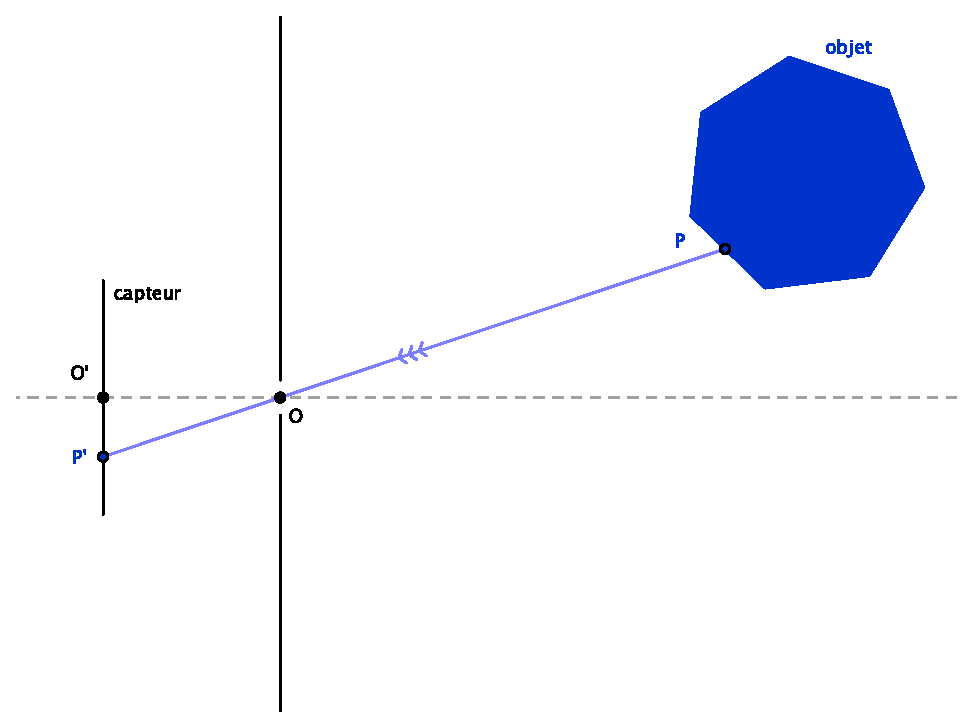
\includegraphics[width=.6\textwidth]{pinhole.eps}
\caption{Modèle caméra pin-hole}
\label{fig:pinhole}
\end{figure}


\subsection{Calibrage}
La calibrage en photogrammétrie consiste à estimer les paramètres extrinsèques et/ou intrinsèques d'une caméra en utilisant une ou plusieurs photo d'un objet (pattern de calibrage) connu. \cite{Truc1998} Figure \ref{fig:calibration_pattern} montre un exemple d'un ``polygone de calibrage'' utilisé dans un laboratoire de recherche. \cite{Gard2009} Plusieurs cibles se trouvent sur l'objet qui peuvent être repérés sur les photos manuellement ou possiblement par des algorithmes de détection de zones d'intérêt. Les coordonnées 3D de chaque cible sont connus. En comparant les positions 2D des cibles sur plusieurs photos, un calibrage des paramètres extrinsèques et intrinsèques a pu été effectué dans ce projet.

\begin{figure}[p]
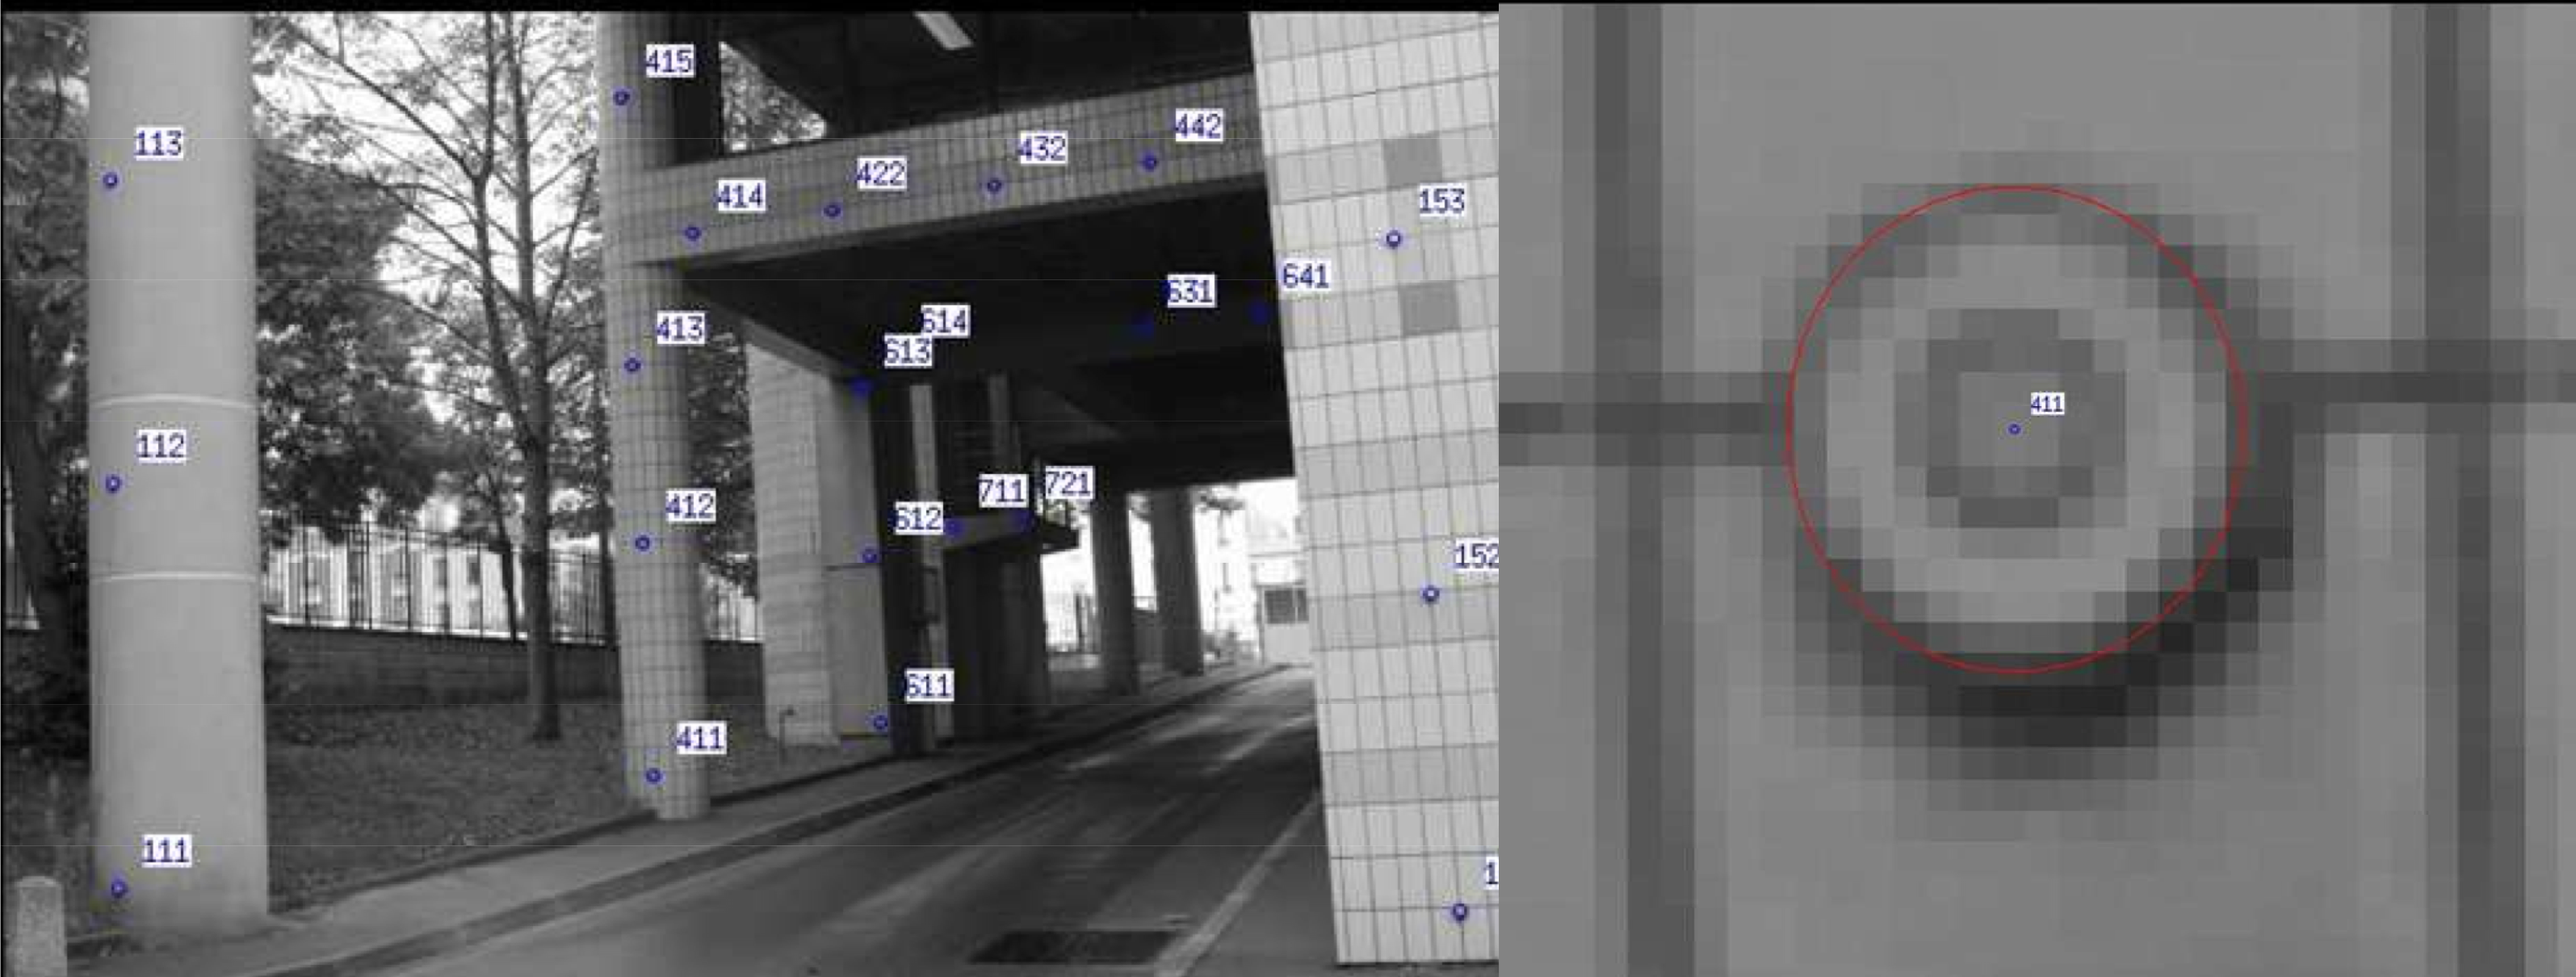
\includegraphics[width=\textwidth]{calibration_pattern.png}
\caption{Exemple de pattern de calibrage utilisé en photogrammétrie. Copié de \cite{Gard2009}}
\label{fig:calibration_pattern}
\end{figure}

La plupart des techniques photogrammétriques supposent que les paramètres extrinsèques et intrinsèques correspondant aux photos sont connus. Sauf si on travaille dans des conditions très particulières (par exemple avec un banc optique où les paramètres sont fixés), il est donc nécessaire d'effectuer un calibrage avant de procéder. Cependant, il existe aussi des techniques qui permettent d'extraire de l'information à partir de photos non-calibrés. \cite{Truc1998}




\subsection{Combination photo-nuage de points}
Comme mentionné, dans des projets de documentation 3D on combine souvent des scans laser avec des information extraits de photos prises en combinaison avec les scans laser. Par exemple cela est usuellement utilisé pour coloriser un nuage de points. Une opération fondamentale est de pouvoir déterminer la position 3D qui correspond à chaque pixel de l'image.

Une technique est décrite dans \cite{Tour2009}. Ici, on suppose que la position et pose de la caméra par rapport au scanner laser est connue.


\chapter{Projet prévu pour le mémoire}



\bibliographystyle{authordate1}
\bibliography{../references}

\end{document}
